\documentclass{article}
% translate with >> pdflatex -shell-escape <file>

% This file is an extract of the PGFPLOTS manual, copyright by Christian Feuersaenger.
% 
% Feel free to use it as long as you cite the pgfplots manual properly.
%
% See
%   http://pgfplots.sourceforge.net/pgfplots.pdf
% for the complete manual.
%
% Any required input files (for <plot table> or <plot file> or the table package) can be downloaded
% at
% http://www.ctan.org/tex-archive/graphics/pgf/contrib/pgfplots/doc/latex/
% and
% http://www.ctan.org/tex-archive/graphics/pgf/contrib/pgfplots/doc/latex/plotdata/

\usepackage{pgfplots}
\pgfplotsset{compat=newest}

\pagestyle{empty}

\usepgfplotslibrary{ternary}

\begin{document}
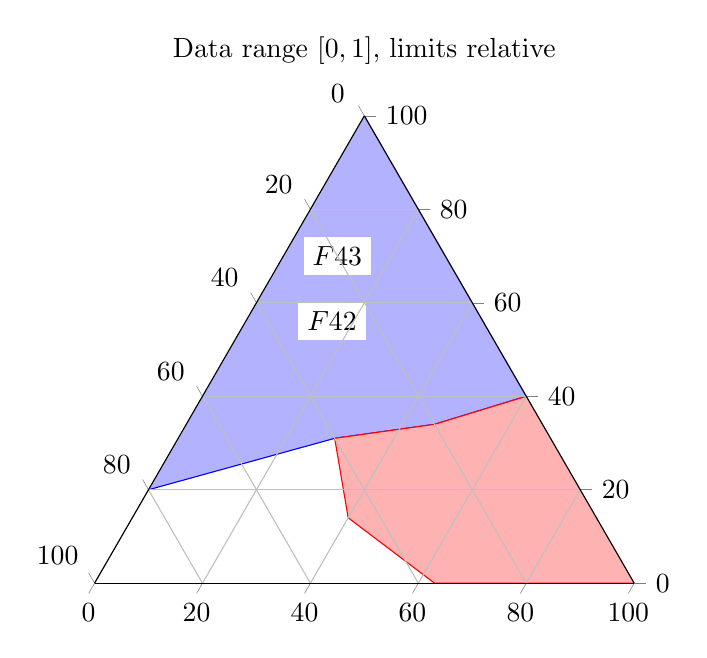
\begin{tikzpicture}
\begin{ternaryaxis}[
	ternary limits relative,
	title={Data range $[0,1]$, limits relative},
	area style]
\addplot3 coordinates {
	(0.2,0.8,0)
	(0.31,0.4,0.29)
	(0.34,0.2,0.46)
	(0.4,0,0.6)
	(1,0,0)
};
\addplot3 coordinates {
	(0.4,0,0.6)
	(0.34,0.2,0.46)
	(0.31,0.4,0.29)
	(0.14,0.46,0.4)
	(0,0.37,0.63)
	(0,0,1)
};
\node[fill=white] 
	at (axis cs:0.56,0.28,0.16) {$F 42$};
\node[fill=white] 
	at (0.7,0.2) {$F 43$};
\end{ternaryaxis}
\end{tikzpicture}
\end{document}
